\documentclass[11pt]{article}

\usepackage[margin=1in]{geometry}
\usepackage{amsmath,amsfonts,amssymb}
\usepackage[none]{hyphenat}
\usepackage{fancyhdr}

\usepackage{multicol}
\usepackage{graphicx}
\usepackage{pgfplots}
\usepackage{wrapfig}

\pagestyle{fancy}
\fancyhead{}
\fancyfoot{}
\fancyhead[L]{\slshape \MakeUppercase{1.1 - Four Ways to Represent a Function}}
\fancyhead[R]{\slshape Ho Ngoc Van}
\fancyfoot[C]{\thepage}
\renewcommand{\footrulewidth}{0pt}

\newcommand{\vct}{\mathbf}
\newcommand{\matx}{\mathbf}
\newcommand{\tens}{\mathsf}
\newcommand{\set}{\mathbb}

\begin{document}
	
\section*{Problem 1}

\textit{If $f(x)=x+\sqrt{2-x}$ and $g(x)=u+\sqrt{2-u}$, is it true that $f=g$?}

\subsection*{Solution}

True


\section*{Problem 2}

\textit{If $$f(x)=\frac{x^2-x}{x-1} \quad\mathrm{and}\quad g(x)=x$$ is it true that $f=g$?}

\subsection*{Solution}

False

\section*{Problem 3}

\textit{The graph of a function $g$ is given:}

\begin{figure}[h]
	\centering
	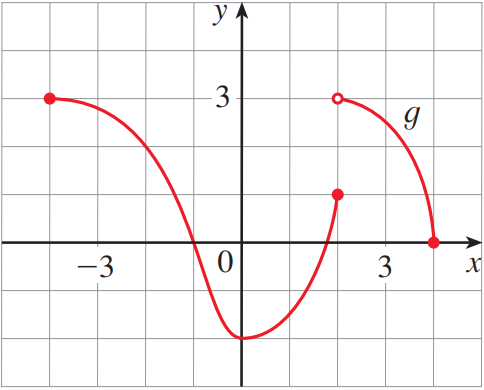
\includegraphics[width=0.3\linewidth]{figs/1.1.3}
\end{figure}

\begin{enumerate}
	\item \textit{State the values of $g(-2)$, $g(0)$, $g(2)$ and $g(3)$}
	\subsection*{Solution}
	$g(-2)=2 \quad g(0)=-2 \quad g(2)=1 \quad g(3)=2.5$
	
	\item \textit{For what value(s) of $x$ is $g(x)=3$?}
	\subsection*{Solution}
	$g(x)=3 \Rightarrow x=-4$
	
	\item \textit{For what value(s) of $x$ is $g(x) \leq 3$?}
	\subsection*{Solution}
	$g(x) \leq 3 \Rightarrow x \in [-4,4]$
	
	\item \textit{State the domain and range of $g$}
	\subsection*{Solution}
	$\mathrm{Domain}:[-4,4] \qquad\mathrm{Range}:[-2,3]$
	
	\item \textit{On what interval(s) is $g$ increasing?}
	\subsection*{Solution}
	$[0,2]$
\end{enumerate}

\end{document}
